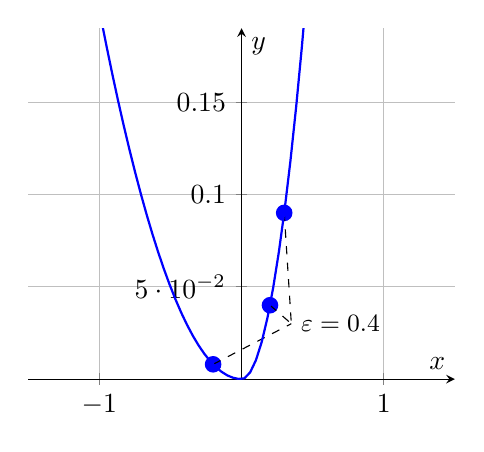
\begin{tikzpicture}[
  declare function={
    func(\x)= (\x < 0) * (x*x/5)   +
              (\x >= 0) * (x*x)
   ;
  }
]
\begin{axis}[
    width=7cm,
    xlabel={$x$},
    ylabel={$y$},
    xmin=-1.5, xmax=1.5,
    ymin=0, ymax=0.19, % Adjust y-axis limits
    axis lines=center,
    grid=both,
    domain=-2:2,
    samples=100,
    % restrict y to domain=-2.5:2.5 % Restrict y-axis domain
]

\coordinate (A1) at (axis cs:-0.2,0.008);
\coordinate (A2) at (axis cs:0.2,0.04);
\coordinate (A3) at (axis cs:0.3,0.09);

\coordinate (B1) at (axis cs:0.35,0.03);

\fill[blue, thick] (A1) circle (3pt);
\fill[blue, thick] (A2) circle (3pt);
\fill[blue, thick] (A3) circle (3pt);


\node[right] at (B1) {\small $\bm{\varepsilon = 0.4}$};

\draw[dashed] (A1) -- (B1);
\draw[dashed] (A2) -- (B1);
\draw[dashed] (A3) -- (B1);

\addplot [blue,thick] {func(x)};
\end{axis}
\end{tikzpicture}